

\section{Experiments and Analysis}





\subsection{Chalearn LAP Data Set \& Evaluation Metrics} \label{sec:chalearn}
The data set\footnote{\href{http://gesture.chalearn.org/homewebsourcereferrals}{http://gesture.chalearn.org/homewebsourcereferrals}} used in this work is provided by the ChaLearn LAP \cite{chalearnLAP} gesture spotting challenge. The development set consists of 700 video sequences and 240 sequences are used for testing. The testing sequences however are not segmented a priori and the gestures must be detected within a continuous data stream. In total, there are more than $14\,000$ performed gestures.
% This dataset  is on ``multiple instance, user independent learning and continuous gesture spotting"~\cite{ICMI} of gestures.
% In the 3 track, there are more than 14,000 gestures.

For the input sequences, there are three modalities provided, \emph{i.e.} skeleton, RGB and depth images (with user segmentation). In the following experiments, the first 650 videos equences are used for training, 50 for validation and the other 240 for testing where each sequence contains around 10 to 20 gestures with some noisy non-meaningful vocabulary tokens.

The evaluation of this data set is performed using the Jaccard index, which computes the overlap between the ground truth and the predictions on a frame-by-frame basis:
\begin{equation}
J(A, B) = \frac{A \bigcap B}{A \bigcup B}
\end{equation}
where $A$ is the ground truth gesture label and $B$ is the predicted gesture label.


\begin{figure*}[t]
        \centering
        \begin{subfigure}[c]{.8\textwidth}
                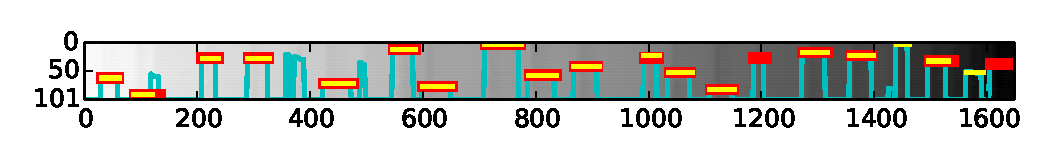
\includegraphics[width=\textwidth]{images/path/Sample0700_sk}
                \caption{Sample \#700 skeleton input path.}
                \label{Sample0700_sk}
        \end{subfigure}%
        ~ %add desired spacing between images, e. g. ~, \quad, \qquad, \hfill etc.
          %(or a blank line to force the subfigure onto a new line)

        \begin{subfigure}[c]{0.8\textwidth}
                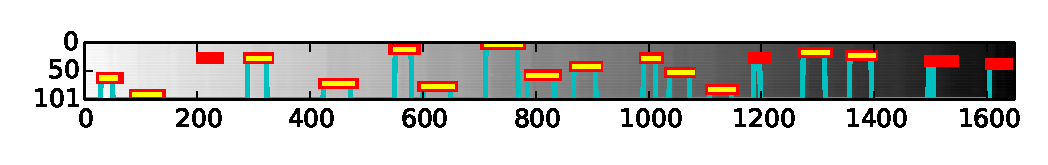
\includegraphics[width=\textwidth]{images/path/Sample0700_cnn}
                \caption{Sample \#700 depth and RGB input path.}
                \label{Sample0700_cnn}
        \end{subfigure}

        ~ %add desired spacing between images, e. g. ~, \quad, \qquad, \hfill etc.
          %(or a blank line to force the subfigure onto a new line)
        \begin{subfigure}[c]{0.8\textwidth}
                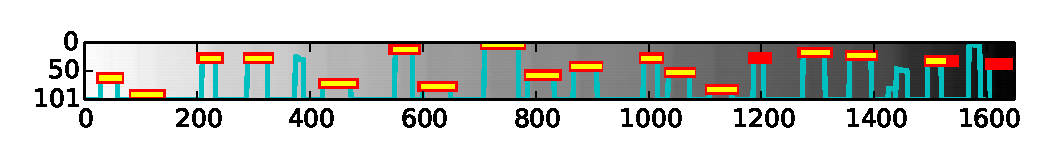
\includegraphics[width=\textwidth]{images/path/Sample0700_combined}
                \caption{Sample \#700 combined input path.}
                \label{Sample0700_combined}
        \end{subfigure}

  \caption{Viterbi decoding of the two modules and their fusion of sample sequence \#700. Top to bottom: skeleton, RGBD, multimodal fusion with x-axis representing the time and y-axis representing the hidden states of all the classes with the ergodic state at the bottom. Red lines are the ground truth labels, cyan lines represent the viterbi shortest path and yellow lines are the predicted labels. There are some complementary information of the two modules and generally the skeletal module outperforms the depth module. The fusion of the two could exploit the uncertainty, \emph{e.g.} around frame 200 the skeleton can help with the false negative predictions given by the 3DCNN module. Around frame 1450, the 3DCNN module can help suppress the false positive prediction given by skeleton module.
  }\label{Sample0700_comparison}
\end{figure*}

\subsection{Post-processing}
The predicted tokens that happen to be less than 20 frames are discarded as noisy tokens. Note that there are many noisy gesture tokens predicted by viterbi decoding. One way to sift through the noisy tokens is to discard the token path log probability smaller than a certain threshold. However, because we use the Jaccard index as evaluation score, it strongly penalises false negatives. Experiments show that the evaluation metric favours having more false positives than missing true positives. Effective ways to detect false positives should be an interesting aspect of future work.

\subsection{Results}

The individual module results and the fusion results are shown in Tab. \ref{Table_score_fusion}. Note that the skeleton module generally performs better than the depth module, one reason could be that the skeleton joints learnt from~\cite{shotton2011real} lie in success of utilising huge and highly varied training data: from both realistic and synthetic depth images, a total number of 1 million images were used to train the deep randomised decision forest classifier in order to avoid overfitting. Hence, skeleton data is more robust.

From the frame based prediction, we also evaluate the gesture token classification rate using the commonly-used PASCAL overlap criterion: if the gesture is predicted correctly with more than 50\% overlap with the ground truth label, then the prediction is counted as a true positive. The results of the two individual modules and the score of the fused modules are shown in Tab.~\ref{Prediction}. From the confusion matrices in Fig.~\ref{confusion_matrix} we can observe the complimentary information between the skeleton input and the RGBD input.
% with the confusion matrices shown in Fig.~\ref{confusion_matrix}.
While many of the gestures in this data set could be mainly differentiated by examining the positions and motions of large joints such as the elbows and wrists,  some gestures differ primarily  in hand pose, \emph{e.g.} Fig. \ref{hand_differ}.
% From the confusion matrices in Fig.~\ref{confusion_matrix} we can observe the complimentary information between the skeleton input and the depth \& RGB input.
%%%%%%%%%%%%%%%%%%%%%%%%%%%%%%%%%%%%%%%%%%%%%%%%%%%%%%%%%%
%%%%%%%%%%%%%%%%%%%%%%%%%%%%%%%%%%%%%%%%%%%%%%%%%%%%%%%%%%
 \begin{table}[t]
   \centering
        \begin{tabular}{|l||*{2}{c|}}\hline
            {Module}
            &\makebox[5em]{Validation}&\makebox[5em]{Test}
            \\\hline\hline
            {\small Skeleton -- DBDN }            &  0.78266    & 0.77920 \\\hline
            {\small RGBD -- 3DCNN }      &  0.75163    & 0.71678 \\\hline%\hline
            {\small Multimodal Late Fusion }              &  0.81744    & 0.80910 \\\hline
            {\small Multimodal Early Fusion }             &  0.80014    & 0.79800 \\\hline
        \end{tabular}

    \caption{
    Comparison of results in terms of Jaccard index between different network structures and various modules.
          }
          \label{Table_score_fusion}
\end{table}
%%%%%%%%%%%%%%%%%%%%%%%%%%%%%%%%%%%%%%%%%%%%%%%%%%%%%%%%%%


%%%%%%%%%%%%%%%%%%%%%%%%%%%%%%%%%%%%%%%%%%%%%%%%%%%%%%%%%%

 \begin{table}[rt]
   \centering
        \begin{tabular}{|ll||*{2}{c|}}\hline
            %\backslashbox{Module}{Evaluation Set}
             & &  \makebox[5em]{Validation}&\makebox[5em]{Test}       \\\hline\hline
            \multirow{2}{*}{Skeleton}       &{\small Acc}                & 0.8633     & 0.8360\\
                                            &  {\small UnRate}           & 0.0230     & 0.0412 \\\hline\hline
            \multirow{2}{*}{RGBD}    &{\small Acc }              & 0.7871     & 0.7581  \\
                                            &  {\small UnRate}           & 0.1612     & 0.1976 \\\hline\hline
            \multirow{2}{*}{Multimodal Late Fusion}   &{\small Acc }               & 0.8791     & 0.8642\\
                                            &  {\small UnRate}           & 0.0302     & 0.0485 \\\hline
           \multirow{2}{*}{Multimodal Early Fusion}   &{\small Acc }    & 0.8650     & 0.8545\\
                                            &  {\small UnRate}           & 0.0623     & 0.0768 \\\hline
        \end{tabular}

    \caption{
    Gesture classification accuracy (\emph{Acc}) and undetected rate (\emph{UnRate}): if the prediction overlaps with the ground truth with more than 50\%, it's considered a true positive.
          }
          \label{Prediction}
\end{table}

%%%%%%%%%%%%%%%%%%%%%%%%%%%%%%%%%%%%%%%%%%%%%%%%%%%%%%%%%%
%%%%%%%%%%%%%%%%%%%%%%%%%%%%%%%%%%%%%%%%%%%%%%%%%%%%%%%%%%
\begin{figure}[t]
        \centering
        \begin{subfigure}[c]{.36\textwidth}
                \includegraphics[width=\textwidth]{images/cm/cm_sk}
                \caption{Skeletal input prediction result.}
                \label{sk_cm}
        \end{subfigure}%
        ~ %add desired spacing between images, e. g. ~, \quad, \qquad, \hfill etc.
          %(or a blank line to force the subfigure onto a new line)

        \begin{subfigure}[c]{0.36\textwidth}
                \includegraphics[width=\textwidth]{images/cm/cm_cnn}
                \caption{RGBD input prediction result.}
                \label{cnn_cm}
        \end{subfigure}

        ~ %add desired spacing between images, e. g. ~, \quad, \qquad, \hfill etc.
          %(or a blank line to force the subfigure onto a new line)
        \begin{subfigure}[c]{0.36\textwidth}
                \includegraphics[width=\textwidth]{images/cm/cm_combination}
                \caption{Multimodal fusion prediction result.}
                \label{fusion_cm}
        \end{subfigure}

  \caption{Confusion Matrix for the skeletal input, RGBD input and multimodal fusion result.
  % Generally, the skeleton module has higher classification rate.
  Some gestures, \emph{e.g.} ``OK" and ``Non ce ne piu" differ primarily in hand poses. Hence, they are easier to be differentiated using the RGBD module than the skeleton module.
  }\label{confusion_matrix}
\end{figure}
%%%%%%%%%%%%%%%%%%%%%%%%%%%%%%%%%%%%%%%%%%%%%%%%%%%%%%%%%%

\begin{figure}[t]
        \centering


        \begin{subfigure}[c]{.2\textwidth}
        \centering
                \includegraphics[width=3cm,height=3cm, trim=120 100 100 50, clip]{images/good}
                \caption{Well-recognised}
        \end{subfigure}%
        %
        \begin{subfigure}[c]{0.2\textwidth}
        \centering
                \includegraphics[width=3cm,height=3cm, trim=120 100 100 50, clip]{images/bad}
                \caption{Poorly-recognised}
        \end{subfigure}
  \caption{
  Examples of overall upper body movement's influence on system performance. Left (score: 0.94) performer almost kept static upper body whilst performing Italian sign language. Right (score: 0.34) performer moved vehemently when performing the gestures.
  }\label{good_bad_differ}
\end{figure}



\begin{figure}[t]
        \centering


        \begin{subfigure}[c]{.2\textwidth}
        \centering
                \includegraphics[width=2cm,height=3cm, trim=120 100 100 50, clip]{images/ok}
                \caption{``OK"}
        \end{subfigure}%
        %
        \begin{subfigure}[c]{0.2\textwidth}
        \centering
                \includegraphics[width=2cm,height=3cm, trim=120 100 100 50, clip]{images/noncenepiu}
                \caption{``Non ce ne piu"}
        \end{subfigure}
  \caption{Examples of gestures that differ primarily in hand pose but not the arm motions.
  }\label{hand_differ}
\end{figure}

%%%%%%%%%%%%%%%%%%%%%%%%%%%%%%%%%%%%%%%%%%%%%%%%%%%%%%%%%%%%
 \begin{table}[t]
   \centering
        \begin{tabular}{|l||*{3}{c|}}\hline
            \backslashbox{Module}{Evaluation Set}
            &\makebox[3em]{Skeleton}&\makebox[6em]{RGBD}&\makebox[3em]{Fusion}
            \\\hline\hline
            {~\cite{neverova2014multi}} Deep Learning (Step 4)                  &   0.7891     &  0.7990      & \textbf{0.8449}\\\hline
            {~\cite{neverova2014multi}} Deep Learning (multiscal)               &   0.8080     &  0.8096      & \textbf{ 0.8488}\\\hline
            {~\cite{Monnier2014multi}} 3 Set Skeletal \& HOG                   &   0.791     & -           & 0.8220 \\\hline
            {~\cite{Chang2014multi}}   Handcrafted features                       &  \textbf{0.7948}     & -           & 0.8268\\\hline
            {~\cite{Peng2014multi}}    Dense Trajectory                         &  -          & \textbf{0.7919}      & -\\\hline
            {~\cite{lio2014deep}}      CNN                                      &  -          & 0.7888      & -\\\hline
            {~\cite{wu2014deep}}    Deep Learning                               &  0.7468     & 0.6371      & 0.8045\\\hline \hline
            \textbf{\emph{DDNN}} (this work)                                    &  0.7792    & 0.7168  & 0.8091\\\hline
        \end{tabular}
    \caption{
    Comparison of results in terms of Jaccard index between different network structures and various modules.
          }
          \label{Table_baseline}
\end{table}

\subsection{Computational Complexity}\label{Computational Complexity}
Although training the deep neural network using stochastic gradient descent is computationally intensive, once the model finishes training, our framework can perform real-time video sequence labelling with a low inference cost.
Specifically, a single feed forward neural network incurs linear computational time ($\mathcal{O}(T)$) and is efficient because it requires only matrix products and convolution operations. The complexity of the Viterbi algorithm is $\mathcal{O} (T* |S|^2)$ with $T$ the number of frames and $|S|$ the number of states.

Using a modern GPU (GeForece GTX TITAN Black), our multimodal neural network can be deployed at 90 FPS using Theano library~\cite{Bastien-Theano-2012} which is 6 times of real time (15 FPS). The preprocessing part takes most of the time and our un-optimized preprocessing pipeline is 25 FPS and Viterbi decoding is 90 FPS. Hence, the overall system can achieve faster than real-time performance.





\endinput
